\chapter{Resultados}

\section{Prueba inicial revisada por señales de simulador}

En primera instancia es importante seleccionar señales que permitan verificar que el funcionamiento del dispositivo es el correcto, y que ejerciten las operaciones descritas anteriormente en la implementación del método de Newton-Raphson.

Se corrieron 32 pruebas con distintas variaciones en los bancos de prueba, donde se dividían 4 pruebas, para cada conjunto de iteraciones de 1 hasta 4 en el método de Newton-Raphson, relacionadas a un subconjunto de entrada que va de 8 bits hasta los 15 bits. Los bancos de prueba en la componente de chequeo guardaban los datos que luego se procesaron por medio de un programa en python que convirtió que calcula el error real que se había producido por medio de la Unidad de Generación de Rayos.

En esta sección del trabajo se muestran dos capturas de pantalla que corresponden a ciertas vistas del simulador que emplea el ISE de Xilinx, mostrando las etapas de una iteración del método de Newton-Raphson en el cálculo del inverso de la raíz cuadrada del número 2 en formato de punto fijo con escala 17.

En la imagen 1 se muestra en wA el valor de entrada correspondiente a 0x400000 que equivale a 2 en representación de punto fijo con la coma corrida 17 espacios hacia la izquierda. Se observa como en la primera instrucción el valor del registro de salida rResult toma el valor 0x16A09 que corresponde al valor de aproximación que provee la tabla de valores iniciales. De hecho el número 0x16A09 equivale en números reales aproximadamente a 0.7070999, esto se sabe al traducir 0x16A09 a decimal y después dividirlo entre $2^{17}$, ya en este caso la escala es igual a 17.  

En la tabla \ref{tab:nombres} se pueden apreciar información básica de las señales, con el objetivo de mejorar la comprensión de las señales vistas en el simulador.

% Table generated by Excel2LaTeX from sheet 'Hoja1'
\begin{table}[htbp]
  \centering
  \caption{Información básicas de señales en el simulador}
    \begin{tabular}{rr}
    \toprule
    Señales importantes & Importancia \\
    \midrule
    wA    & Valor del Registro A dentro del RGU \\
    wB    & Valor del Registro B dentro del RGU \\
    wDestination & Número de registro que se escribe en memoria  \\
    wOperation & Código que identifica cada instrucción \\
    rResult & Registro con el valor de salida del RGU \\
    \bottomrule
    \end{tabular}%
  \label{tab:nombres}%
\end{table}%

\begin{figure}
	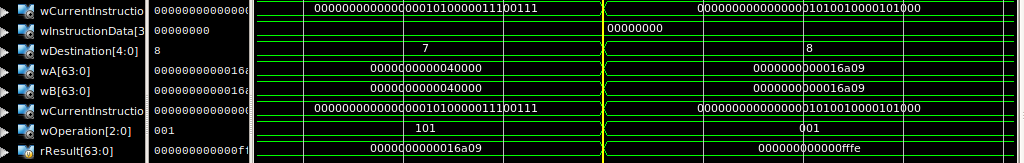
\includegraphics[width=1\linewidth, height=2.5cm]{images/Selection_010}
	\caption{Primera parte de captura de la simulación de señales} \label{fig:sim1}
\end{figure}

En la imagen 1 se pueden seguir viendo las operaciones que corresponden a los pasos intermedios de multiplicación por los que pasa.

En la imagen 2 se observa que después de realizar las operaciones de multiplicación, resta y desplazamiento se obtiene que en la última operación el registro rResult adquiere el valor de 0x16A0A, equivalente a 0.7071075, lo cual implica que la iteración respecto al valor ini mejoró la aproximación del inverso de la raíz cuadrada pues el valor real es aproximadamente 0.7071067. Lo anterior implica la tendencia de mejorar la precisión siempre y cuando se encuentre un valor inicial cercano al valor meta. 

\begin{figure}
	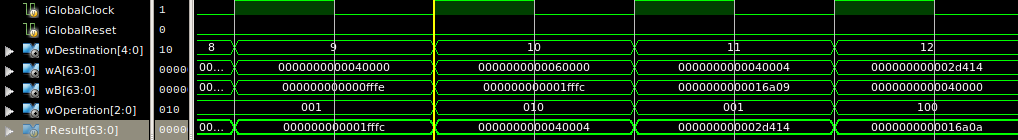
\includegraphics[width=1\linewidth, height=2.5cm]{images/Selection_011}
	\caption{Segunda parte de captura de la simulación de señales} \label{fig:sim2}
\end{figure}

\section{Pruebas en los distintos rangos de bits de entrada}

El  RGU puede tener hasta 15 bits de parte entera pero tiene una tabla de memoria con 128 valores (7 bits) para generar una valor de iteración inicial, entonces se implementó un módulo llamado FixedPointSquareRoot cuya capacidad es aumentar el rango de cobertura de la unidad, pero dicho módulo aumenta el error al hacer una estimación ya que hace un corrimiento hacia la derecha de los 8 bits menos significativos de la parte entera de los números de entrada en formato de punto fijo para poder encontrar un valor en la tabla que abarca solo números de 7 bits (128 posibilidades).

Entonces sucede que existe una gran variabilidad respecto a los porcentajes de error dependiendo de los rangos mayores a 7 bits, por ejemplo los casos que son de 8 bits en la primera iteración provocan errores de casi el 50 porciento mientras que los casos de 12 bits poseen un error inferior al 1 porciento ante estímulos seudoaleatorios.

\begin{figure}
	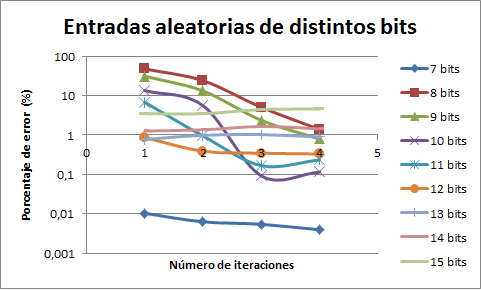
\includegraphics[width=0.7\linewidth]{images/puntos}
	\caption{Gráfico sobre los porcentajes de error ante iteraciones con distintos rangos de bits} \label{fig:puntos}
\end{figure}

En el caso de la figura \ref{fig:puntos}, cuya escala en el eje Y es logarítmica, se puede observar, por ejemplo, que con tres iteraciones el comportamiento de las entradas con 10 bits de parte entera cambia mucho y para una cuarta iteración queda literalmente en la misma posición, lo cual implicaría que más de tres iteraciones en realidad no es necesario para obtener un margen de error apropiado para ese número de iteraciones.

En general la tendencia de las entradas con distintos bits es disminuir su porcentaje de error conforme se van aumentando las iteraciones. Solo en los casos de 14 y 15 bits se puede apreciar que se pierde el cáracter de disminución observado en los casos de menor cantidad de bits y más bien se genera un error casi constante, lo cual estaría dado por la incapacidad del hardware de proporcionar valores iniciales más precisos para lo cual se necesitaría tablas con mayor cantidad de valores.

En la tablas \ref{tab:errores1} y \ref{tab:errores2} se pueden observar que los porcentajes de error en 8 y 9 bits al iniciar las iteraciones eran bastante altos pero conforme se iteraba se alcanzaba un porcentaje de error más bajo.  

Lo que sucede es que para valores de solo 8 y 9 bits el error inicial es mucho ya que siempre se está haciendo un corrimiento de 8 bits a la parte entera del número. 

% Table generated by Excel2LaTeX from sheet 'Hoja1'
\begin{table}[htbp]
  \centering
  \caption{Tabla de iteraciones de 7 a 12 bits de entrada con su respectivo error}
    \begin{tabular}{rrrrrrrrr}
    \toprule
    Iteración     & 7     & 8     & 9     & 10    & 11    & 12\\
    \midrule
    1    & 0,01031246 & 47,7288136 & 31,2230569 & 13,3993714 & 6,78690633 & 0,86304167\\
    2    & 0,00627204 & 23,9909933 & 13,1553409 & 5,56002376 & 0,94484015 & 0,38862163\\
    3    & 0,00542083 & 5,05170113 & 2,36331935 & 0,09193496 & 0,16717202 & 0,34528176\\
    4    & 0,00393699 & 1,39280231 & 0,79338167 & 0,11496986 & 0,23323379 & 0,32996335\\
    \bottomrule
    \end{tabular}%
  \label{tab:errores1}%
\end{table}% 


% Table generated by Excel2LaTeX from sheet 'Hoja1'
\begin{table}[htbp]
  \centering
  \caption{Tabla de iteraciones de 7 a 12 bits de entrada con su respectivo error}
    \begin{tabular}{rrrrrrrrr}
    \toprule
    Iteración     & 13    & 14    & 15 \\
    \midrule
    1    &    0,77210039 & 1,26359914 & 3,47221991 \\
    2    &    0,98878366 & 1,35671632 & 3,47967437 \\
    3    &    1,0228597 & 1,65155714 & 4,43548373 \\
    4    &    0,89261429 & 1,42975391 & 4,55886896 \\
    \bottomrule
    \end{tabular}%
  \label{tab:errores2}%
\end{table}% 
%%%%%%%%%%%%%%%%%%%%%%%%%%%%%%%%%%%%%%%%%%%%%%%%%%%%%%%%%%%%%%%%%%%%%%%%%%%%%%%%%%%%%%%%%%%%%%%%%%%%%%%%%%%%
%%%%%%%%%%%%%%%%%%%%%%%%%%%%%%%%%%%%%%%%%%%%%%%%%%%%%%%%%%%%%%%%%%%%%%%%%%%%%%%%%%%%%%%%%%%%%%%%%%%%%%%%%%%%
%%%%%%%%%%%%%%%%%  MACHOTE  %%%%%%%%%%%%%%%%%%%%%%%%%%%%%%%%%%%%%%%%%%%%%%%%%%%%%%%%%%%%%%%%%%%%%%%%%%%%%%%%
%%%%%%%%%%%%%%%%%%%%%%%%%%%%%%%%%%%%%%%%%%%%%%%%%%%%%%%%%%%%%%%%%%%%%%%%%%%%%%%%%%%%%%%%%%%%%%%%%%%%%%%%%%%%
%%%%%%%%%%%%%%%%%%%%%%%%%%%%%%%%%%%%%%%%%%%%%%%%%%%%%%%%%%%%%%%%%%%%%%%%%%%%%%%%%%%%%%%%%%%%%%%%%%%%%%%%%%%%
\begin{comment}


\section{Pruebas para comprobar la funcionalidad y estabilidad}

Al finalizar el desarrollo de la aplicación, se probó acceder a ella desde computadoras en diferentes sistemas operativos. En todos los casos la aplicación operaba de forma correcta. Por lo que independientemente del OS del sistema, la herramienta es funcional, dando como resultado una aplicación web, multiplataforma. Lo cual era uno de los objetivos que se quería alcanzar inicialmente.\\

Además se analizó la exactitud de los datos obtenidos. A la hora de realizar los contornos con la herramienta desarrollado, siempre se obtuvo todos los pixeles que forman parte del mismo, distinto a Sensarea que se obtenían muy pocos puntos si se realizaba la funcionalidad de esta misma manera (dejando precionado el click izquierdo y desplazando el puntero al rededor del contorno).


\section{Pruebas realizadas por diversos usuarios}

Para probar que la aplicación diseñada en efecto es más sencilla de utilizar que las otras herramientas actuales y que con ella se generan datos de manera más eficiente, se procedió a realizar unas pruebas con tiempo a tres diferentes usuarios y se promedió el resultado. Las otras dos herramientas con las cuales se comparó fueron Sensara y VideoANT, debido a que son las únicas que no se requiere de conocimiento técnico para poder instalarlas o utilizarlas en línea. A cada uno se les solicitó realizar las siguientes tareas en orden:

\begin{enumerate}
\item Instalar o acceder a la aplicación
\item Abrir la aplicación, cargar uno de sus video y realizar la segmentación temporal de 5 escenas diferentes.
\item Seguir de la trayectoria de 5 elementos diferentes por al menos 20 cuadros.
\item Dibujar los contornos de 5 elementos diferentes por al menos 20 cuadros.
\item Realizar anotaciones semánticas de 5 tipos diferentes de escenas encontradas.
\end{enumerate}

El video que se utilizó fue una sección de la final de la Copa del Mundo Fifa 2010 entre España y Holanda. El peso del video es de 250 Mb, el formato es mp4 y codec es h264. Los resultados obtenidos se muestran en las tablas \ref{table:results} y \ref{table:results2}. La primera de ellas muestra lo que se duró haciendo la labor por primera vez y en la segunda tabla se muestra el valor promedio de tiempos en las 5 tareas de cada tipo.


\begin{table}[h]\centering
	
	\ra{2}
	\caption{Promedio de tiempo estimado de la primera función realizada correctamente}
	\label{table:results}
	
	\begin{tabular}{@{}cC{3cm}C{3cm}C{3cm}C{3cm}c@{}}\toprule
		
		& Función & GT-Tool & Sensarea & VideoANT&\\ \midrule
		
		& Primer uso de la aplicación & 7 segundos* & 2 minutos & 5 segundos* & \\
		
		& Segmentación temporal  & 26 segundos & 87 segundos & 15 segundos & \\
		
		& Rastreo de objetos & 5 segundos & 5 segundos & no aplica & \\
		
		& Segmentación de contornos & 27 segundos  & 34 segundos & no aplica & \\
		
		& Segmentación semántica & 20 segundos  & no aplica & 15 segundos & \\ 
		
		\bottomrule
		
	\end{tabular}
	
\end{table}

*Ese el tiempo que les tomó acceder a la página web, de lo contrario es el tiempo de descarga e instalación.\\

Se puede apreciar de esta primera tabla (\ref{table:results}), que GT-Tool es muy similar a Sensarea cuando se quiere realizar el seguimiento de la trayectoria de los objetos. Y es un poco más lento que VideoANT a la hora de realizar la segmentación temporal y semántica, esto es debido a la forma en la que VideoANT solicita la información, es más directa pero no tan especializada. De nuevo, VideoANT da precisión de segundos y no de cuadros y además no tiene manera de realizar seguimiento de trayectorias ni segmentación de contornos.\\

A continuación el promedio de las 5 repeticiones luego de haber realizado la tarea por primera vez:


\begin{table}[h]\centering
	
	\ra{2}
	\caption{Promedio de tiempo que tomó realizar cada función repetidas veces (5 repeticiones)}
	\label{table:results2}
	
	\begin{tabular}{@{}cC{3cm}C{3cm}C{3cm}C{3cm}c@{}}\toprule
		
		& Función & GT-Tool & Sensarea & VideoANT&\\ \midrule
		
		& Segmentación temporal  & 19 segundos & 30 segundos & 13 segundos & \\
		
		& Rastreo de objetos & 3 segundos & 4 segundos & no aplica & \\
		
		& Segmentación de contornos & 14 segundos  & 29 segundos & no aplica & \\
		
		& Segmentación semántica & 15 segundos  & no aplica & 13 segundos & \\ 
		
		\bottomrule
		
	\end{tabular}
	
\end{table}

Al analizar los resultados de dicha tabla se concluye los siguiente:

\begin{enumerate}
	
\item A medida que utilizan cualquier herramienta, el tiempo que les toma realizar una labor disminuye, sin importar cual sea. La disminución más grande la tuvo Sensarea en la segmentación temporal, pero esto fue debido a que, aunque Sensarea no soporta nativamente algún tipo de segmentación temporal, se puede simular colocando puntos con etiquetas. Cuando los usuarios se dieron cuenta de esto, lo empezaron a hacer y así hacían un tipo de segmentación temporal.

\item VideoANT continua siendo un poco más rápida para lo temporal y semántico, pero no cuenta con los otros tipos. De igual manera la diferencia en tiempos no es muy significativa.

\item GT-Tool si logra disminuir el tiempo en el que se generan los datos para la trayectoria de objetos y segmentación de contornos, mientras que a la vez aumenta la precisión brindada por Sensarea.

\end{enumerate}

\end{comment}